\documentclass[11pt,a4paper]{article}
\usepackage[utf8]{inputenc}
\usepackage[T1]{fontenc}
\usepackage[margin=2.2cm]{geometry}
\usepackage{booktabs}
\usepackage{graphicx}
\usepackage{float}
\usepackage{longtable}
\usepackage{fancyhdr}
\usepackage{amsmath,amssymb}
\usepackage{xcolor}
\usepackage[hidelinks]{hyperref}
\setlength{\parindent}{0pt}
\setlength{\parskip}{6pt}
\pagestyle{fancy}\fancyhf{}
\lhead{\small A Multi-Agent Fact-Checking Assistant}
\rhead{\small\thepage}
\renewcommand{\headrulewidth}{0.4pt}
\begin{document}
\begin{center}
{\LARGE\bfseries MAFCA: Results Report}\\[4pt]
{\large A Multi-Agent Fact-Checking Assistant}\\[10pt]
Machine Learning IA 2\\[2pt]
Department of Computer Engineering, K. J. Somaiya School of Engineering, Somaiya Vidyavihar University\\[8pt]
\textbf{Shanu Sharma and Krutika Sadadekar}
\end{center}
\vspace{6pt}\hrule\vspace{10pt}
\section*{Scope and reproducibility}
Every table, figure and number in this document was produced by executing the code in this repository on n = 90 AVeriTeC claims. Nothing is transcribed by hand: each value is read from a generated macro in results/macros/, and a name that no longer exists raises an error rather than printing a blank.
\textbf{To reproduce every artefact below:}
\begin{verbatim}
python src/analysis/regenerate.py      # rebuilds results/ from the cache
python src/analysis/build_results_doc.py   # rebuilds this document
python -m pytest -q                    # 434 tests
\end{verbatim}
This runs offline. It makes no model call and needs no corpus download: the retrieved passages are committed in cache/av250.jsonl and the per-claim verdicts in results/, so the chain replays exactly. Decoding is greedy (temperature 0) and every sampling step is seeded, so reruns reproduce the same values.
Scope: the protocol was designed for 250 claims. The search service degraded partway through retrieval and the run was halted at 90 claims rather than looped, because continuing against a failing endpoint fills the cache with empty evidence sets indistinguishable from genuine 'nothing found' results. This is a pilot, and the statistical power table states what it can and cannot settle.
\clearpage
\section{Console output}
Actual console output from executing the analysis chain. The full files are in logs/ in the repository.
\subsection{Regeneration of every result: \texttt{python src/analysis/regenerate.py}}
\begin{small}\begin{verbatim}
wrote 90 paired records to D:\proj\submission\results\averitec_n90_v2.jsonl
  baseline = B0, multi = MAFCA
  labels: NOT_ENOUGH_INFO 29, REFUTES 25, SUPPORTS 36
n = 90 claims from D:\proj\submission\results\averitec_n90_v2.jsonl

  Single-LLM (existing)      acc  42.2%  macro-F1  39.8%  decidable  24.6%  latency   6.1s
  MAFCA computed (proposed)  acc  48.9%  macro-F1  47.4%  decidable  34.4%  latency  20.6s
  MAFCA agent-reported (ablation) acc  47.8%  macro-F1  45.2%  decidable  29.5%  latency  20.6s

Tables -> results\tables\av_tables.tex
Charts -> results\figures/av_*.png
  retrieval    results\figures/av_retrieval.png
  reliability  results\figures/av_reliability.png
  ablation     results\figures/av_ablation.png

Aggregation ablation  ?  D:\proj\submission\results\averitec_n90_v2.jsonl  ?  n = 90
policy                                      acc    mF1     ECE   Brier  overconf   cited  support
-------------------------------------------------------------------------------------------------
Single-LLM baseline                        42.2   39.8   0.192   0.273     +19.2     0.0      0.0
MAFCA, as run                              47.8   45.2   0.376   0.390      -2.4    66.7     72.7
  + deterministic agg. (beta=0)            48.9   47.4   0.268   0.306      +5.3    38.9    100.0
  + deterministic agg. (beta=1)            48.9   47.4   0.280   0.320      +8.6    38.9    100.0
  + deterministic agg. (beta=2)            48.9   47.4   0.289   0.331     +10.5    38.9    100.0
  + det. agg., gating off                  48.9   47.4   0.280   0.320      +8.6    66.7     67.2

Table -> results\tables\av_ablation.tex
Wrote fig_flowchart.png, fig_summary_bar.png and fig_network.png to results\figures/
wrote 239 macros -> D:\proj\submission\results\macros\numbers.tex
  Av: D:\proj\submission\results\averitec_n90_v2.jsonl (90 records)
n = 90 claims, conditions: MAJORITY, RANDOM, B0, B1, MAFCA, B4
  tables -> D:\proj\submission\results\tables
  macros -> D:\proj\submission\results\macros\condition_numbers.tex  (142 definitions)
appended 112 macros -> D:\proj\submission\results\macros\condition_numbers.tex

live: 46 wrong of 90 (resampled range 37-55)
  retrieval       60.9%  [ 46.7,  74.5]  n=28
  verification    39.1%  [ 25.5,  53.3]  n=18
  aggregation      0.0%  [  0.0,   0.0]  n=0
  unattributed     0.0%  [  0.0,   0.0]  n=0

oracle: 35 wrong of 90 (resampled range 26-44)
  retrieval        5.7%  [  0.0,  14.6]  n=2
  verification    94.3%  [ 85.4, 100.0]  n=33
  aggregation      0.0%  [  0.0,   0.0]  n=0
  unattributed     0.0%  [  0.0,   0.0]  n=0

B1 attribution possible: False (no per-passage audit recorded)

wrote 17 macros -> D:\proj\submission\results\macros\attribution_numbers.tex
wrote D:\proj\submission\results\figures\poster_accuracy.png  (n = 90 claims)
  B0: single LLM         overall  42.2   decidable  24.6
  B1: single-call RAG    overall  44.4   decidable  27.9
  MAFCA                  overall  48.9   decidable  34.4

$ python src/analysis/join_conditions.py --conditions D:\proj\submission\results\av250 --cache D:\pr ...

$ python src/analysis/results_report.py --results D:\proj\submission\results\averitec_n90_v2.jsonl - ...

$ python src/analysis/grounding_figures.py --results D:\proj\submission\results\averitec_n90_v2.json ...

$ python src/analysis/ablation.py --results D:\proj\submission\results\averitec_n90_v2.jsonl --tag a ...

$ python src/analysis/summary_figures.py

$ python src/analysis/paper_numbers.py --averitec D:\proj\submission\results\averitec_n90_v2.jsonl - ...

$ python src/analysis/condition_tables.py --dir D:\proj\submission\results\av250 --cache D:\proj\sub ...

$ python src/analysis/oracle_macros.py --live D:\proj\submission\results\av250 --oracle D:\proj\subm ...

... [regenerate.log continues; full file in logs/regenerate.log]
\end{verbatim}\end{small}
\subsection{Test suite: \texttt{python -m pytest -q}}
\begin{small}\begin{verbatim}
........................................................................ [ 16%]
........................................................................ [ 33%]
........................................................................ [ 49%]
........................................................................ [ 66%]
........................................................................ [ 82%]
........................................................................ [ 99%]
..                                                                       [100%]
434 passed in 12.86s
\end{verbatim}\end{small}
\clearpage
\section{Tables}
\subsection{Classification performance}
\begin{table}[H]
\centering
\small
\caption{Classification performance on all n = 90 claims. Values are percentages with 95\% bootstrap confidence intervals over 10,000 resamples. 'Decidable' restricts to claims whose gold label is SUPPORTS or REFUTES. 'Abstention' is the share answered NOT\_ENOUGH\_INFO.}
\label{tab:classification}
\begin{tabular}{@{}lrrrr@{}}
\toprule
\textbf{Condition} & \textbf{Accuracy (\%)} & \textbf{Macro-F1 (\%)} & \textbf{Decidable (\%)} & \textbf{Abstain (\%)} \\
\midrule
B0: single LLM, no retrieval & 42.2 [32.2, 52.2] & 39.8 [28.7, 49.8] & 24.6 [13.8, 35.3] & 73.3 \\
B1: single-call RAG & 44.4 [34.4, 54.4] & 42.0 [31.1, 52.2] & 27.9 [16.9, 39.4] & 66.7 \\
B4: MAFCA, computed verdict & 48.9 [38.9, 58.9] & 47.4 [36.3, 57.5] & 34.4 [23.0, 46.7] & 61.1 \\
MAFCA: agent-reported (ablation) & 47.8 [37.8, 57.8] & 45.2 [34.4, 55.4] & 29.5 [18.3, 41.3] & 67.8 \\
Majority class & 40.0 [30.0, 50.0] & 19.0 [15.4, 22.2] & 59.0 [46.6, 71.0] & 0.0 \\
Random & 28.9 [20.0, 38.9] & 27.9 [18.9, 36.9] & 26.2 [15.5, 37.7] & 36.7 \\
\bottomrule
\end{tabular}
\par\vspace{2pt}\footnotesize{Every condition replays the identical cached passages, so the comparisons are paired claim for claim.}
\end{table}
\subsection{Paired differences between conditions}
\begin{table}[H]
\centering
\small
\caption{Paired differences in percentage points. Positive favours the first-named condition. p is the exact McNemar test on accuracy. Every interval here contains zero.}
\label{tab:differences}
\begin{tabular}{@{}lrrrrr@{}}
\toprule
\textbf{Comparison} & \textbf{$\Delta$Acc (pp)} & \textbf{95\% CI} & \textbf{p} & \textbf{$\Delta$F1 (pp)} & \textbf{95\% CI} \\
\midrule
B4 vs B0 & +6.7 & [-5.6, 18.9] & 0.377 & +7.6 & [-6.1, 21.8] \\
B4 vs B1 & +4.4 & [-4.4, 13.3] & 0.481 & +5.4 & [-4.7, 15.4] \\
MAFCA vs B0 & +5.6 & [-5.6, 16.7] & 0.424 & +5.4 & [-6.9, 18.3] \\
MAFCA vs B1 & +3.3 & [-5.6, 11.1] & 0.607 & +3.2 & [-6.1, 12.6] \\
\bottomrule
\end{tabular}
\par\vspace{2pt}\footnotesize{No comparison reaches significance at this sample size. See the power table for what the sample could have resolved.}
\end{table}
\subsection{Statistical power}
\begin{table}[H]
\centering
\small
\caption{Statistical power of the paired design. The minimum detectable difference (MDD) is the smallest paired difference this sample could resolve; observed differences smaller than it are uninformative in either direction.}
\label{tab:power}
\begin{tabular}{@{}lrr@{}}
\toprule
\textbf{Quantity} & \textbf{B4 vs B0} & \textbf{MAFCA vs B1} \\
\midrule
Claims (n) & 90 & 90 \\
Discordant pairs & 35.6 & 16.7 \\
Informative pairs & 32 & 15 \\
Minimum detectable difference (pp) & 17.6 & 12.1 \\
\bottomrule
\end{tabular}
\par\vspace{2pt}\footnotesize{A paired test only sees claims the two conditions answer differently, which is why the discordant count, not n, drives power.}
\end{table}
\subsection{Calibration}
\begin{table}[H]
\centering
\small
\caption{Calibration and confidence. ECE is expected calibration error and Brier the quadratic score; for both, lower is better. Computing the confidence from the audit rather than eliciting it does not improve either past the single-LLM baseline.}
\label{tab:calibration}
\begin{tabular}{@{}lrr@{}}
\toprule
\textbf{Condition} & \textbf{ECE} & \textbf{Brier} \\
\midrule
B0: single LLM & 0.192 & 0.273 \\
B1: single-call RAG & 0.272 & 0.343 \\
B4: MAFCA, computed & 0.280 & 0.320 \\
MAFCA: agent-reported & 0.376 & 0.390 \\
Majority class & 0.067 & 0.244 \\
Random & 0.044 & 0.207 \\
\bottomrule
\end{tabular}
\end{table}
\subsection{Citations and cost}
\begin{table}[H]
\centering
\small
\caption{Citation behaviour and cost. 'Cited' is the share of verdicts carrying at least one citation that survives validation: it must name a passage that was genuinely retrieved and that the verification stage labelled in the verdict's direction.}
\label{tab:citations}
\begin{tabular}{@{}lrrr@{}}
\toprule
\textbf{Condition} & \textbf{Cited (\%)} & \textbf{Support (\%)} & \textbf{LLM calls} \\
\midrule
B0: single LLM & 0.0 & 0.0 & 1 \\
B1: single-call RAG & 5.6 & 0.0 & 1 \\
B4: MAFCA, computed & 38.9 & 100.0 & 2 \\
MAFCA: agent-reported & 66.7 & 72.7 & 2 \\
\bottomrule
\end{tabular}
\par\vspace{2pt}\footnotesize{B0 cites nothing because it retrieves nothing. The call count is measured at replay: the Evidence Scout's call is made once during cache construction and does not recur.}
\end{table}
\subsection{Error attribution by stage}
\begin{table}[H]
\centering
\small
\caption{Where incorrect verdicts arise, as a share of all errors, with 95\% bootstrap intervals over 10,000 resamples of the claims. This analysis requires a per-passage record, so it cannot be run on the single-call baseline at all.}
\label{tab:attribution}
\begin{tabular}{@{}lrr@{}}
\toprule
\textbf{Stage} & \textbf{Live retrieval (\%)} & \textbf{Oracle evidence (\%)} \\
\midrule
Retrieval & 60.9 [46.7, 74.5] & 5.7 [0.0, 14.6] \\
Verification & 39.1 [25.5, 53.3] & 94.3 [85.4, 100.0] \\
Aggregation & 0.0 [0.0, 0.0] & 0.0 [0.0, 0.0] \\
\bottomrule
\end{tabular}
\par\vspace{2pt}\footnotesize{Retrieval dominates under live conditions. Substituting the corpus' own annotated evidence inverts the profile. No error is attributable to aggregation in either condition, because the computed policy cannot return a verdict the audit does not support.}
\end{table}
\subsection{Oracle-evidence diagnostic}
\begin{table}[H]
\centering
\small
\caption{Oracle-evidence diagnostic: the same claims with the corpus' annotated evidence substituted for web search. This isolates verification quality from retrieval quality. These are diagnostic figures, not deployable performance.}
\label{tab:oracle}
\begin{tabular}{@{}lrrrr@{}}
\toprule
\textbf{Condition} & \textbf{Accuracy (\%)} & \textbf{Macro-F1 (\%)} & \textbf{Decidable (\%)} & \textbf{ECE} \\
\midrule
B1, live evidence & 44.4 [34.4, 54.4] & 42.0 & 27.9 & 0.272 \\
B1, oracle evidence & 61.1 [51.1, 71.1] & 60.6 & 50.8 & 0.136 \\
MAFCA, live evidence & 47.8 [37.8, 57.8] & 45.2 & 29.5 & 0.376 \\
MAFCA, oracle evidence & 58.9 [48.9, 68.9] & 57.5 & 44.3 & 0.412 \\
\bottomrule
\end{tabular}
\end{table}
\subsection{Effect of oracle evidence}
\begin{table}[H]
\centering
\small
\caption{Effect of substituting annotated evidence, in percentage points, with Holm-Bonferroni adjusted p-values across the three comparisons.}
\label{tab:oracle_gain}
\begin{tabular}{@{}lrrrr@{}}
\toprule
\textbf{Comparison} & \textbf{$\Delta$Acc (pp)} & \textbf{95\% CI} & \textbf{p} & \textbf{p (Holm)} \\
\midrule
B1 oracle vs B1 live & +16.7 & [4.4, 28.9] & 0.017 & 0.050 \\
MAFCA oracle vs MAFCA live & +11.1 & [-1.1, 23.3] & 0.121 & 0.243 \\
MAFCA oracle vs B1 oracle & -2.2 & [-11.1, 6.7] & 0.804 & 0.804 \\
\bottomrule
\end{tabular}
\end{table}
\subsection{Retrieval quality}
\begin{table}[H]
\centering
\small
\caption{Retrieval quality against the corpus' annotated source URLs, at two matching strictnesses. Exact matching requires the same URL; domain matching requires only the same site.}
\label{tab:retrieval}
\begin{tabular}{@{}lrr@{}}
\toprule
\textbf{Measure} & \textbf{Exact URL} & \textbf{Domain} \\
\midrule
Claims scored & 87 & 87 \\
Recall@k (\%) & 1.7 & 9.4 \\
Precision@k (\%) & 0.7 & 4.8 \\
Claims with $\geq$1 hit (\%) & 2.3 & 13.8 \\
Mean gold URLs & 1.79 & 1.66 \\
Mean retrieved & 3.66 & 3.29 \\
\bottomrule
\end{tabular}
\par\vspace{2pt}\footnotesize{The system rarely recovers the exact sources the annotator used; it retrieves contemporaneous material instead, which the ungrounded baseline lacks entirely.}
\end{table}
\subsection{Per-class performance}
\begin{table}[H]
\centering
\small
\caption{Per-class precision, recall and F1 (\%), with class support. This is the confusion structure behind the macro-averaged figures: it shows which labels each system actually gets right.}
\label{tab:per_class}
\begin{tabular}{@{}lrrrrr@{}}
\toprule
\textbf{System} & \textbf{Class} & \textbf{Precision} & \textbf{Recall} & \textbf{F1} & \textbf{Support} \\
\midrule
Single LLM (B0) & SUPPORTS & 87.5 & 19.4 & 31.8 & 36 \\
 & REFUTES & 50.0 & 32.0 & 39.0 & 25 \\
 & NOT\_ENOUGH\_INFO & 34.8 & 79.3 & 48.4 & 29 \\
MAFCA computed & SUPPORTS & 66.7 & 33.3 & 44.4 & 36 \\
 & REFUTES & 52.9 & 36.0 & 42.9 & 25 \\
 & NOT\_ENOUGH\_INFO & 41.8 & 79.3 & 54.8 & 29 \\
MAFCA agent-reported & SUPPORTS & 88.9 & 22.2 & 35.6 & 36 \\
 & REFUTES & 50.0 & 40.0 & 44.4 & 25 \\
 & NOT\_ENOUGH\_INFO & 41.0 & 86.2 & 55.6 & 29 \\
\bottomrule
\end{tabular}
\par\vspace{2pt}\footnotesize{Support is the number of claims carrying that gold label.}
\end{table}
\subsection{Latency}
\begin{table}[H]
\centering
\small
\caption{Mean wall-clock latency per claim, in seconds, measured during the run. Decomposition costs time: the pipeline makes more model calls than the control.}
\label{tab:cost}
\begin{tabular}{@{}lr@{}}
\toprule
\textbf{System} & \textbf{Mean latency (s)} \\
\midrule
Single LLM (B0) & 6.1 \\
MAFCA computed & 20.6 \\
MAFCA agent-reported & 20.6 \\
Ratio, MAFCA to baseline & 3.4 \\
\bottomrule
\end{tabular}
\end{table}
\subsection{Pipeline integrity checks}
\begin{table}[H]
\centering
\small
\caption{Pipeline integrity checks, all enforced in code rather than by prompt. These hold by construction and so do not depend on the sample size.}
\label{tab:integrity}
\begin{tabular}{@{}lr@{}}
\toprule
\textbf{Check} & \textbf{Value} \\
\midrule
Claims evaluated & 90 \\
Mean evidence passages per claim & 3.67 \\
Claims with zero evidence retrieved & 2 \\
Claims issuing two distinct queries (\%) & 90 \\
Verdicts with a complete audit trace (\%) & 90 \\
Audit-schema validity (\%) & 100.0 \\
Leakage: fact-check domains filtered & 11 \\
Leakage: claims still exposed & 13 \\
Leakage rate (\%) & 14.4 \\
Quoted-span rate (\%) & 3.6 \\
Spans checkable against passage text & 153 \\
Span violations & 6 \\
\bottomrule
\end{tabular}
\par\vspace{2pt}\footnotesize{The leakage filter removes the claim's own fact-check article from retrieved evidence, which would otherwise hand the verdict to the system.}
\end{table}
\subsection{Retrieval degradation}
\begin{table}[H]
\centering
\small
\caption{Retrieval degradation during the run. The search service failed partway through and the run was halted rather than looped; these counts record how many claims were affected.}
\label{tab:degraded}
\begin{tabular}{@{}lr@{}}
\toprule
\textbf{Quantity} & \textbf{Claims} \\
\midrule
Claims retrieved before the outage & 90 \\
Claims with degraded retrieval & 16 \\
  of which returned no evidence & 2 \\
  of which returned partial evidence & 14 \\
Claims after excluding degraded retrieval & 74 \\
\bottomrule
\end{tabular}
\par\vspace{2pt}\footnotesize{Reporting the clean subset separately guards against a result that depends on which claims the outage happened to hit.}
\end{table}
\clearpage
\section{Figures}
\begin{figure}[H]
\centering
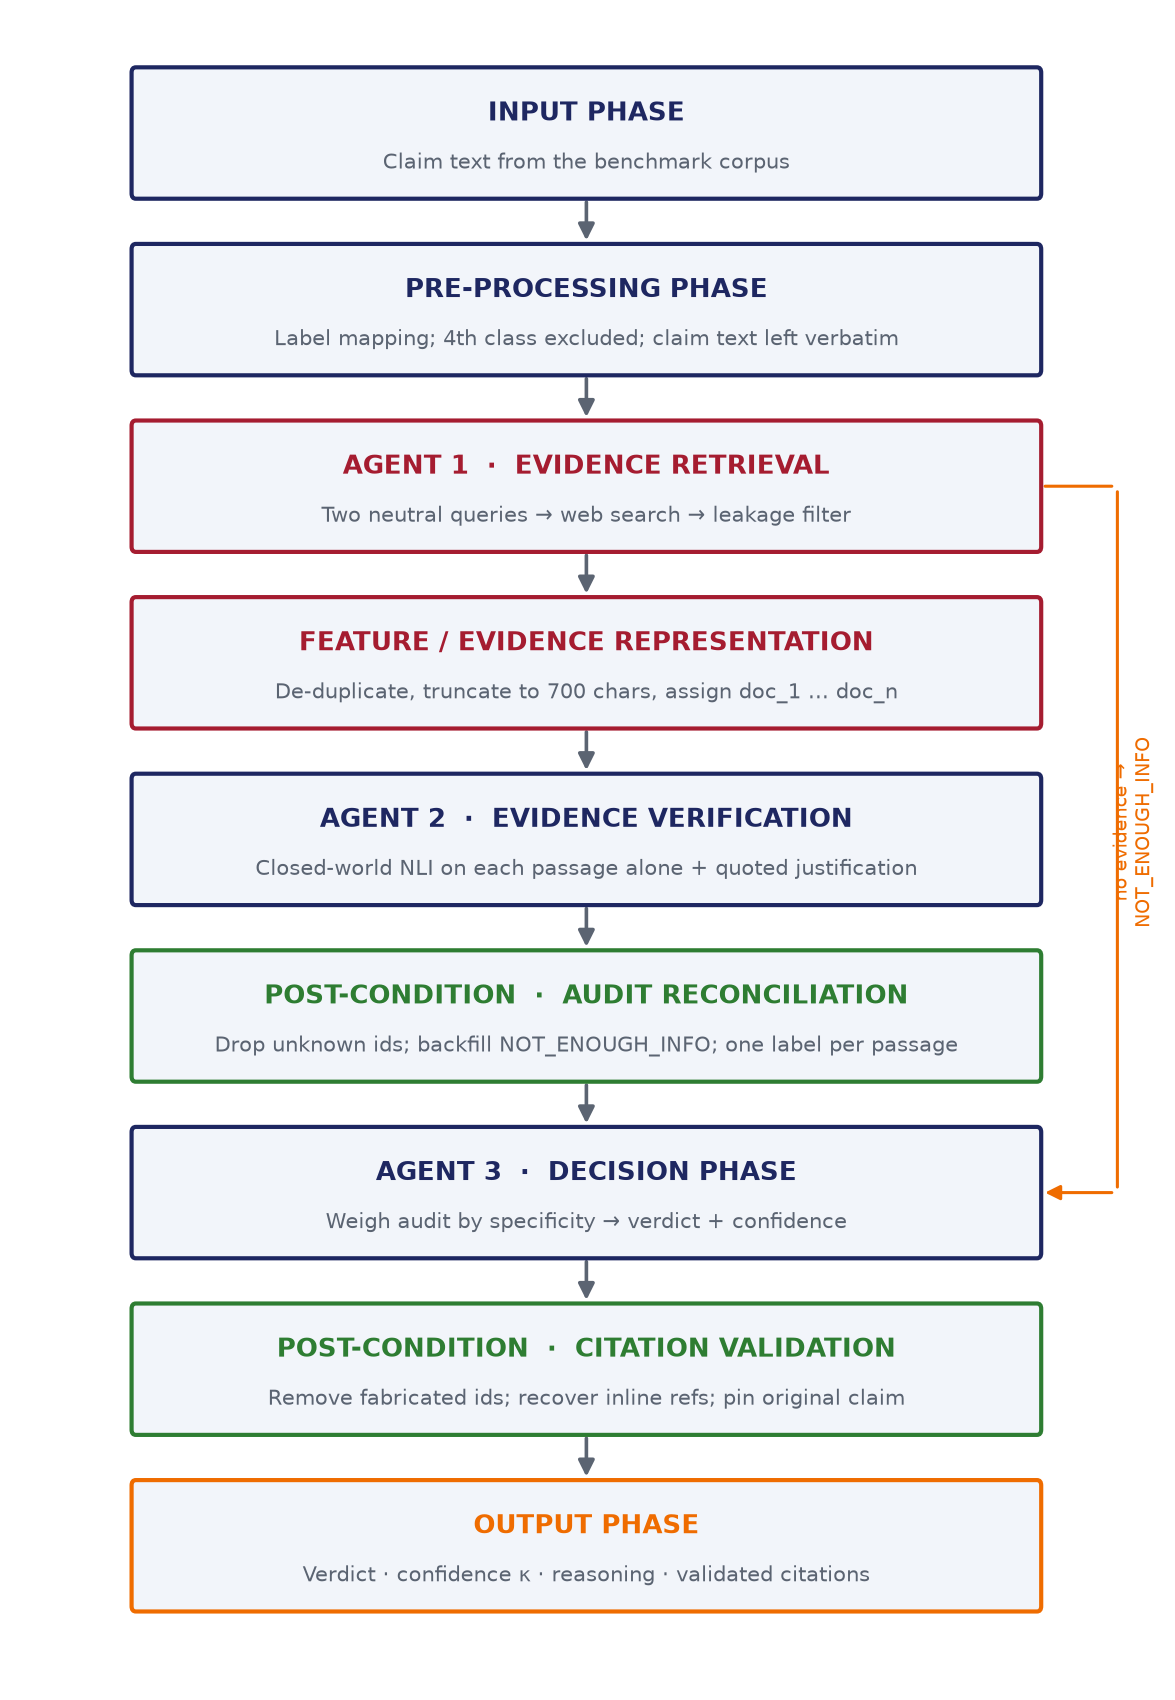
\includegraphics[width=0.84\textwidth]{figures/fig_flowchart.png}
\caption{The three-agent pipeline. Evidence Scout retrieves passages, Alignment Auditor labels each passage separately, and Synthesis Adjudicator writes the reasoning trace while the verdict itself is computed from the audit. \textit{Generated by src/analysis/summary\_figures.py.}}
\end{figure}
\begin{figure}[H]
\centering
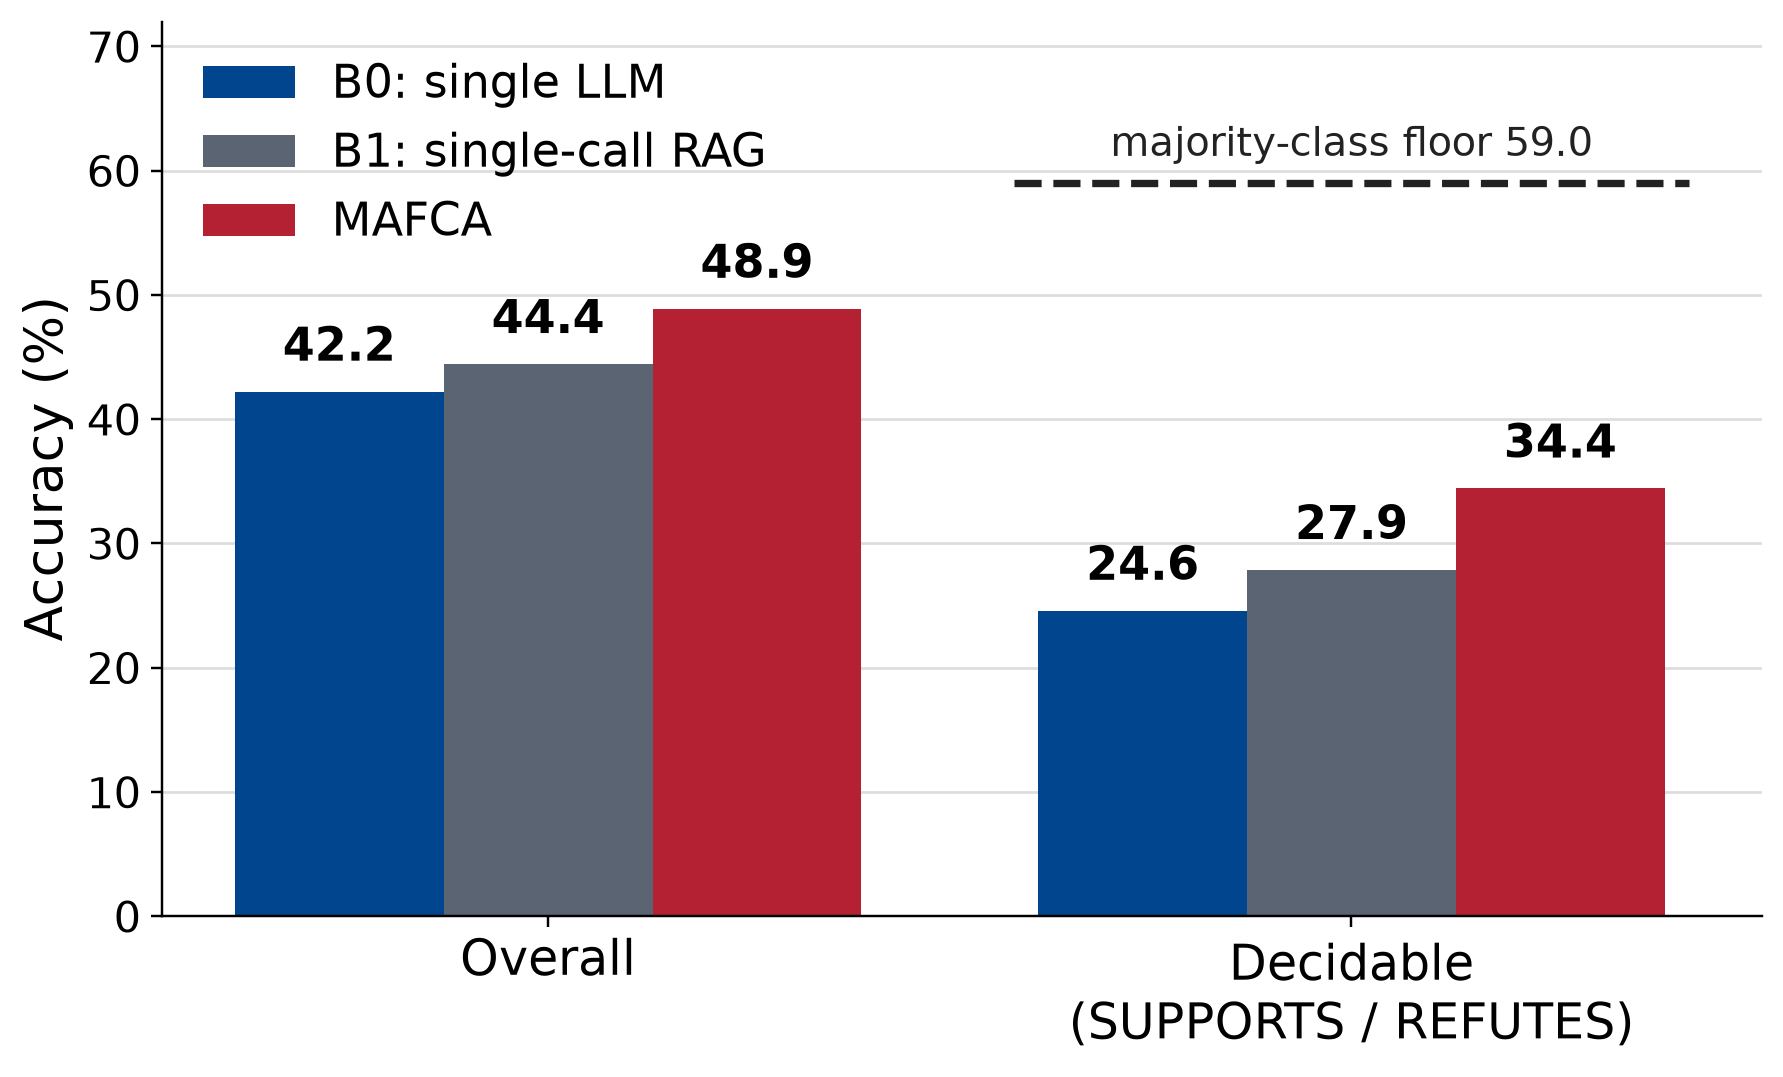
\includegraphics[width=0.84\textwidth]{figures/poster_accuracy.png}
\caption{Accuracy of the single LLM (B0), single-call RAG (B1) and MAFCA, overall and on the decidable subset. The dashed line is the majority-class floor on the decidable subset, which no system reaches. \textit{Generated by src/analysis/poster\_figures.py.}}
\end{figure}
\begin{figure}[H]
\centering
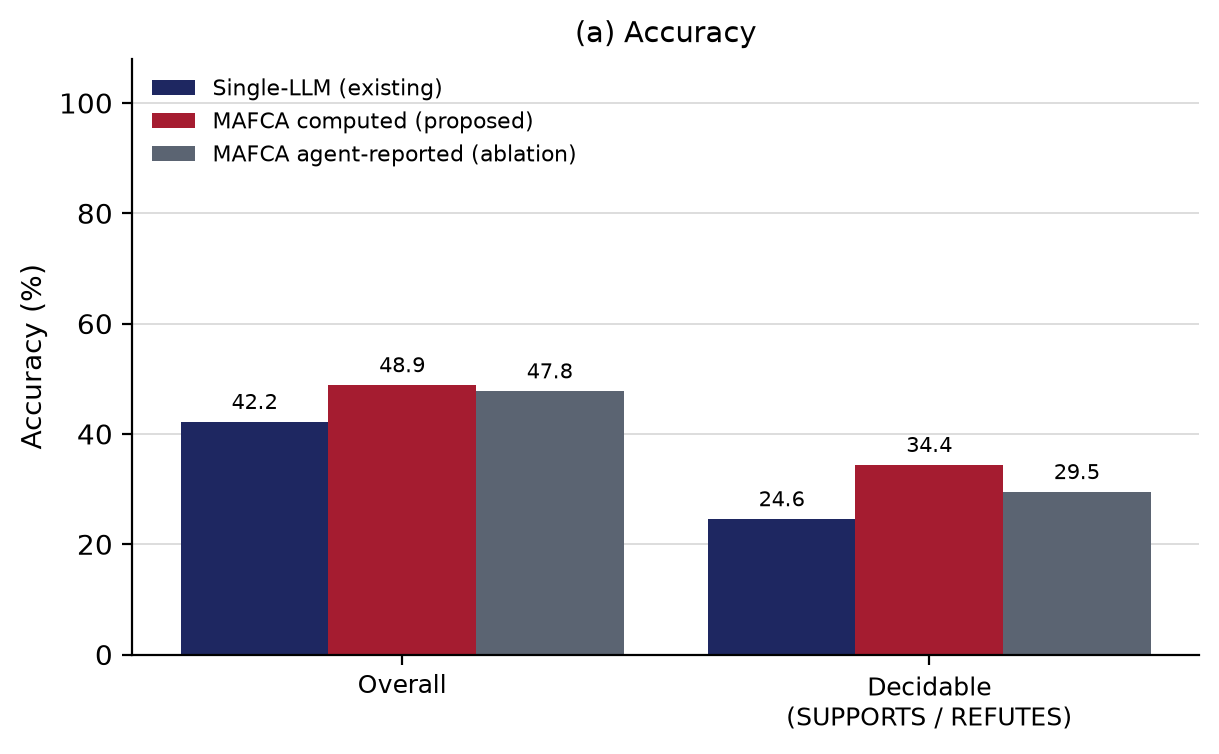
\includegraphics[width=0.84\textwidth]{figures/av_accuracy.png}
\caption{Accuracy, overall and on the decidable subset, for the single-LLM control against both MAFCA configurations. \textit{Generated by src/analysis/results\_report.py.}}
\end{figure}
\begin{figure}[H]
\centering
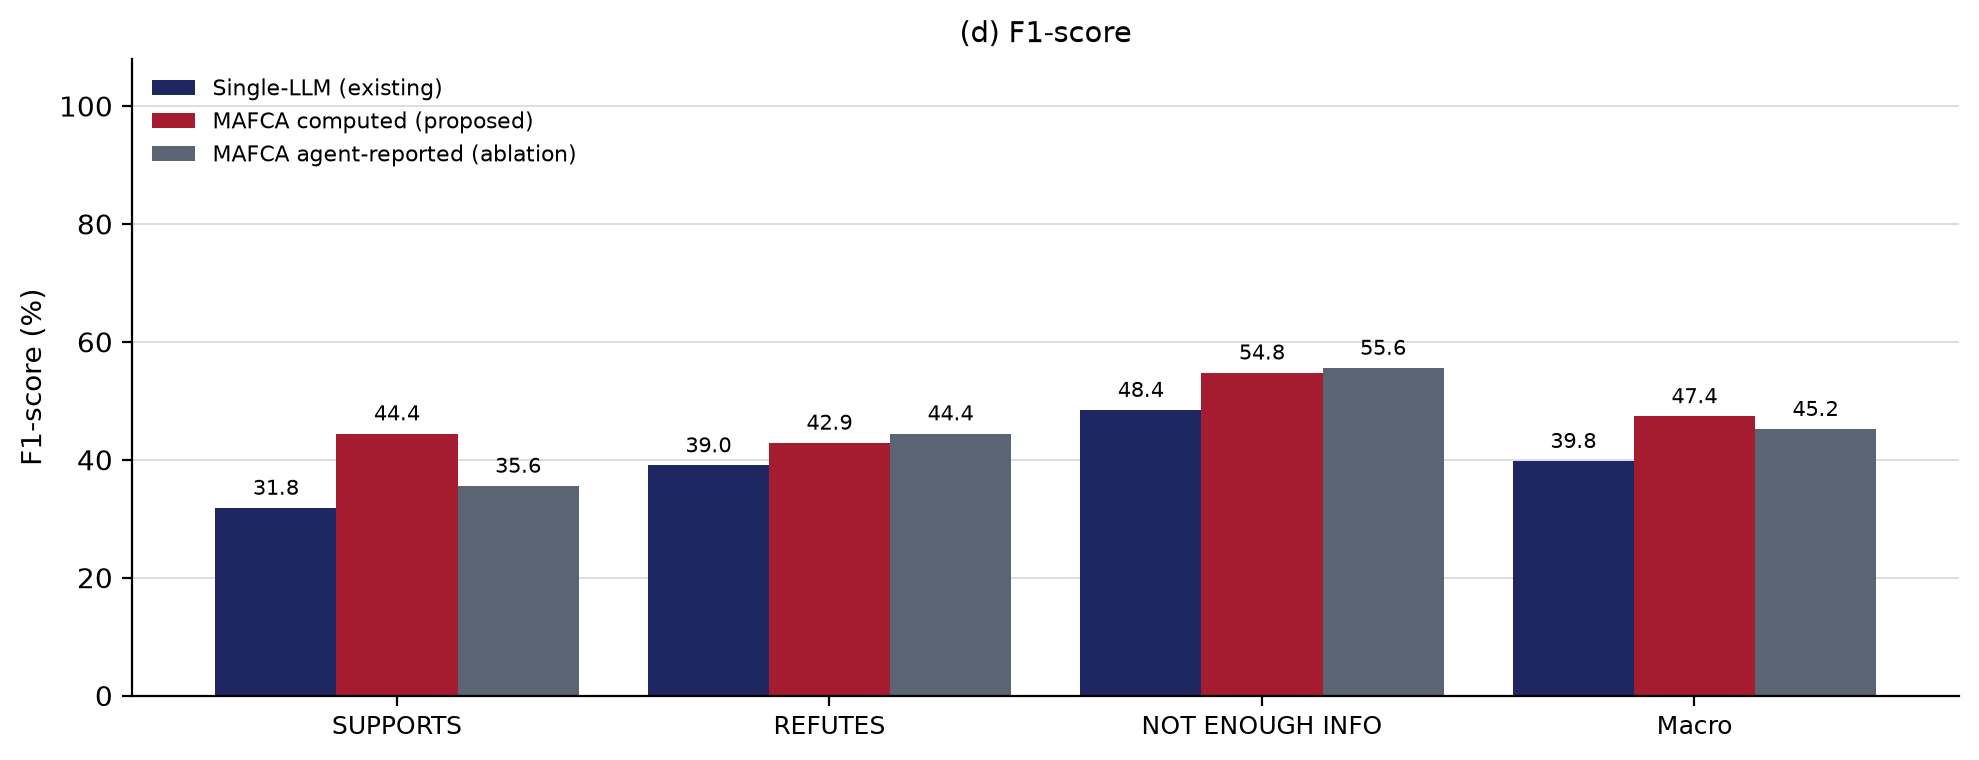
\includegraphics[width=0.84\textwidth]{figures/av_f1.png}
\caption{F1-score by gold label and macro-averaged. \textit{Generated by src/analysis/results\_report.py.}}
\end{figure}
\begin{figure}[H]
\centering
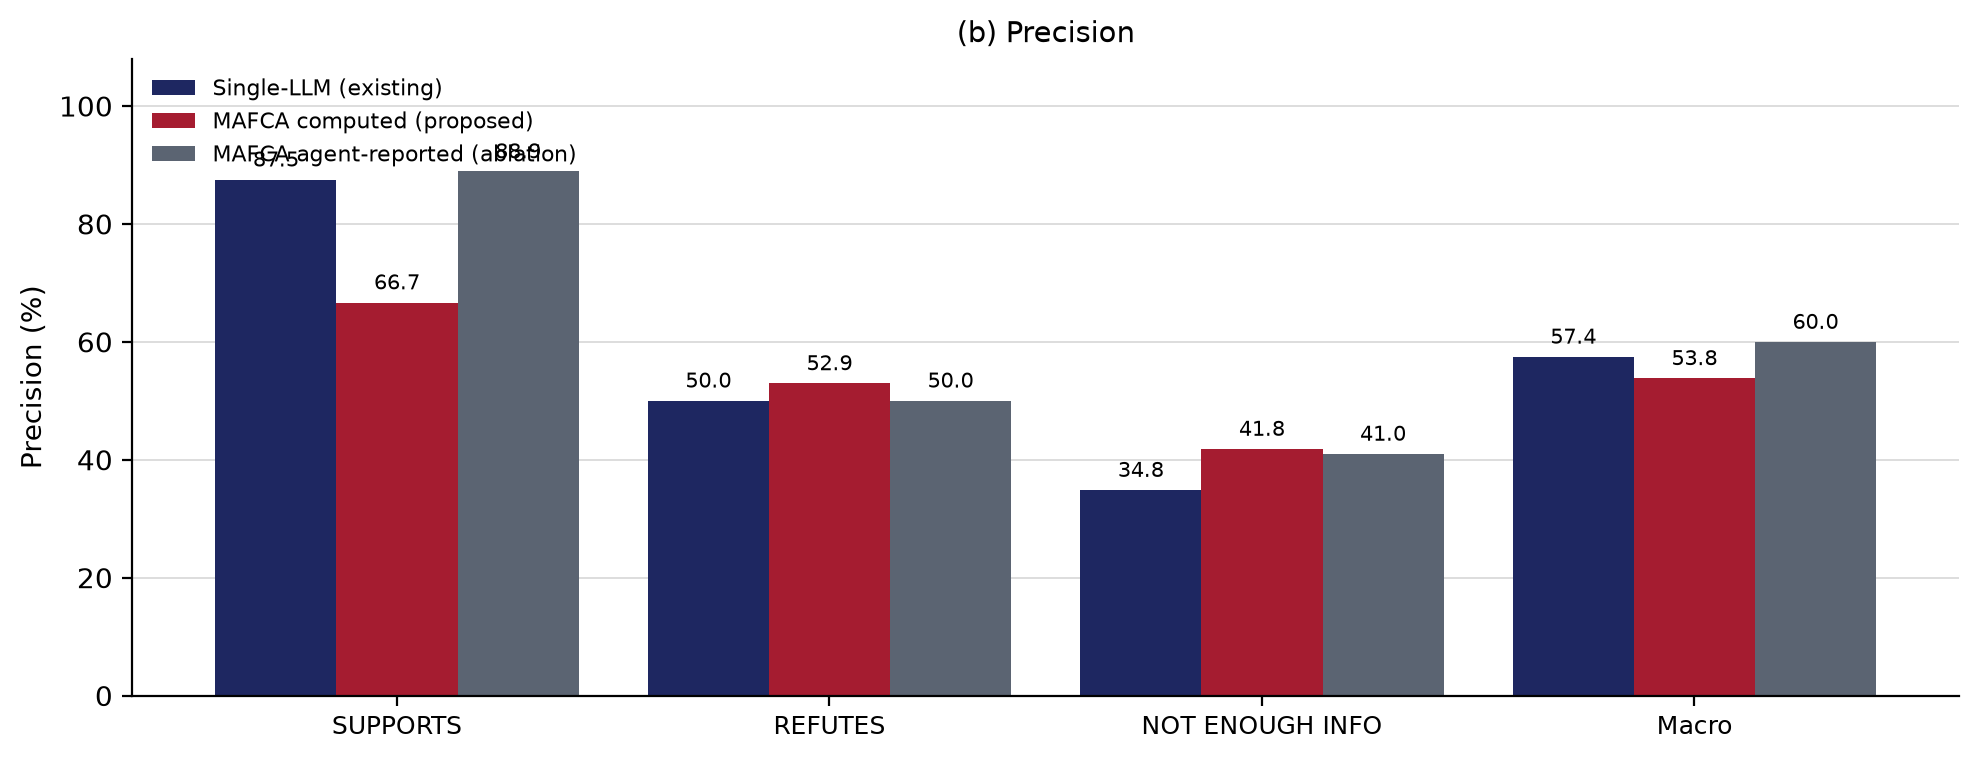
\includegraphics[width=0.84\textwidth]{figures/av_precision.png}
\caption{Precision by gold label and macro-averaged. \textit{Generated by src/analysis/results\_report.py.}}
\end{figure}
\begin{figure}[H]
\centering
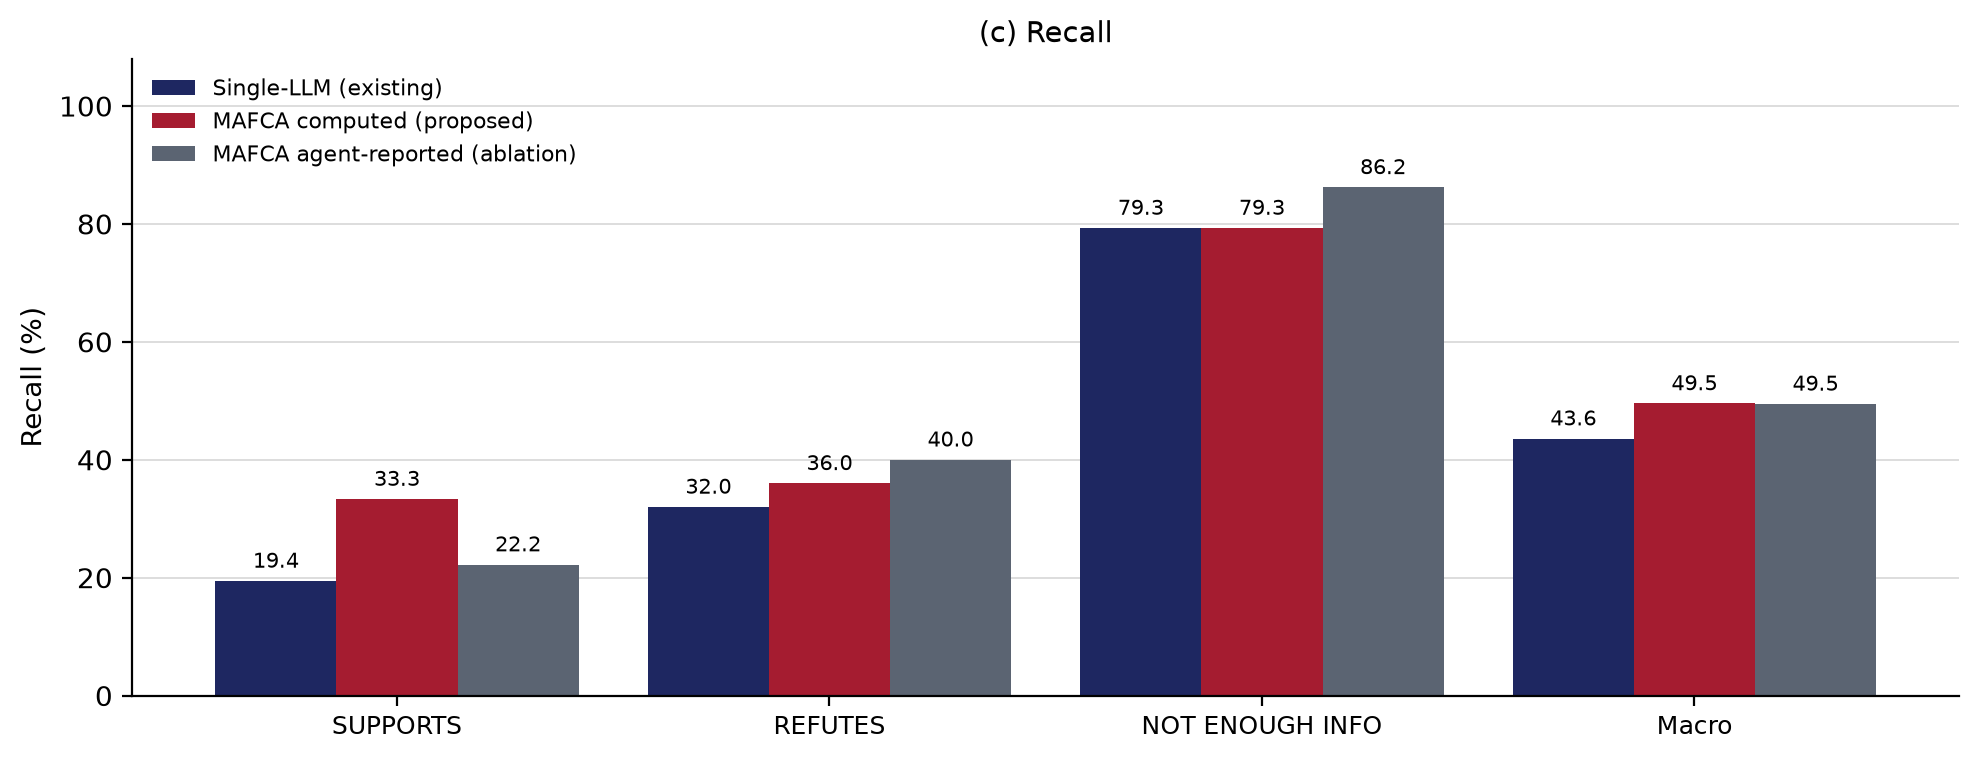
\includegraphics[width=0.84\textwidth]{figures/av_recall.png}
\caption{Recall by gold label and macro-averaged. \textit{Generated by src/analysis/results\_report.py.}}
\end{figure}
\begin{figure}[H]
\centering
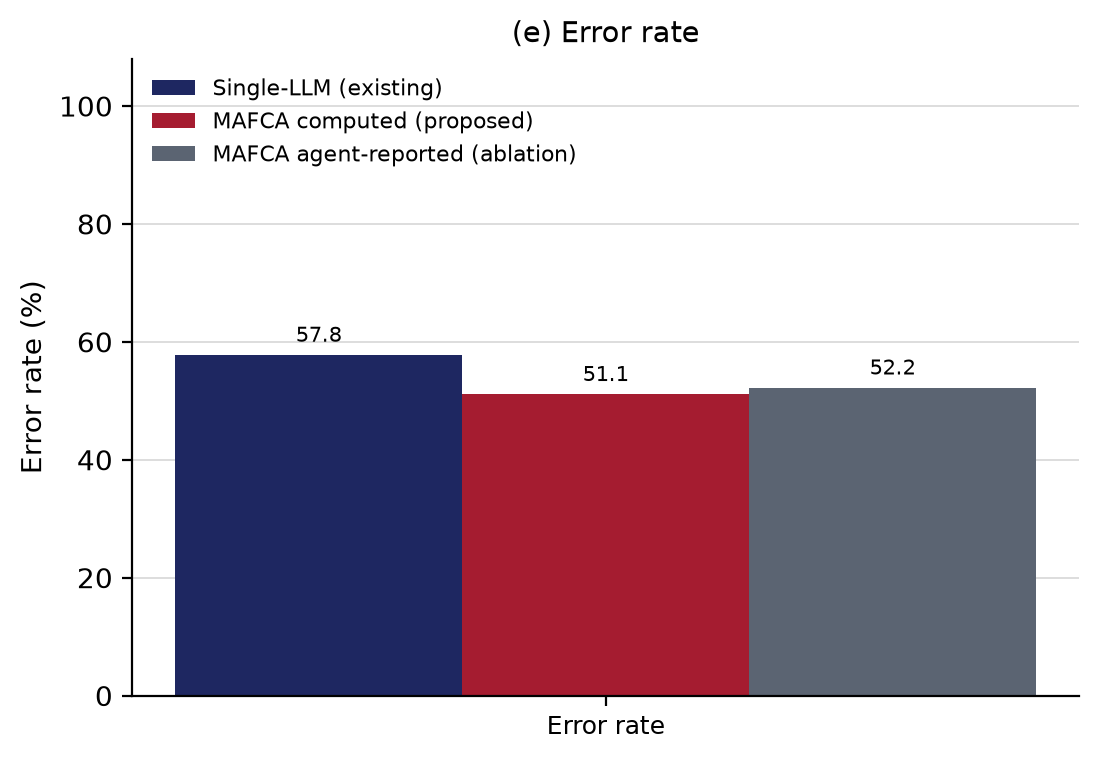
\includegraphics[width=0.84\textwidth]{figures/av_errorrate.png}
\caption{Overall error rate, the complement of accuracy. \textit{Generated by src/analysis/results\_report.py.}}
\end{figure}
\begin{figure}[H]
\centering
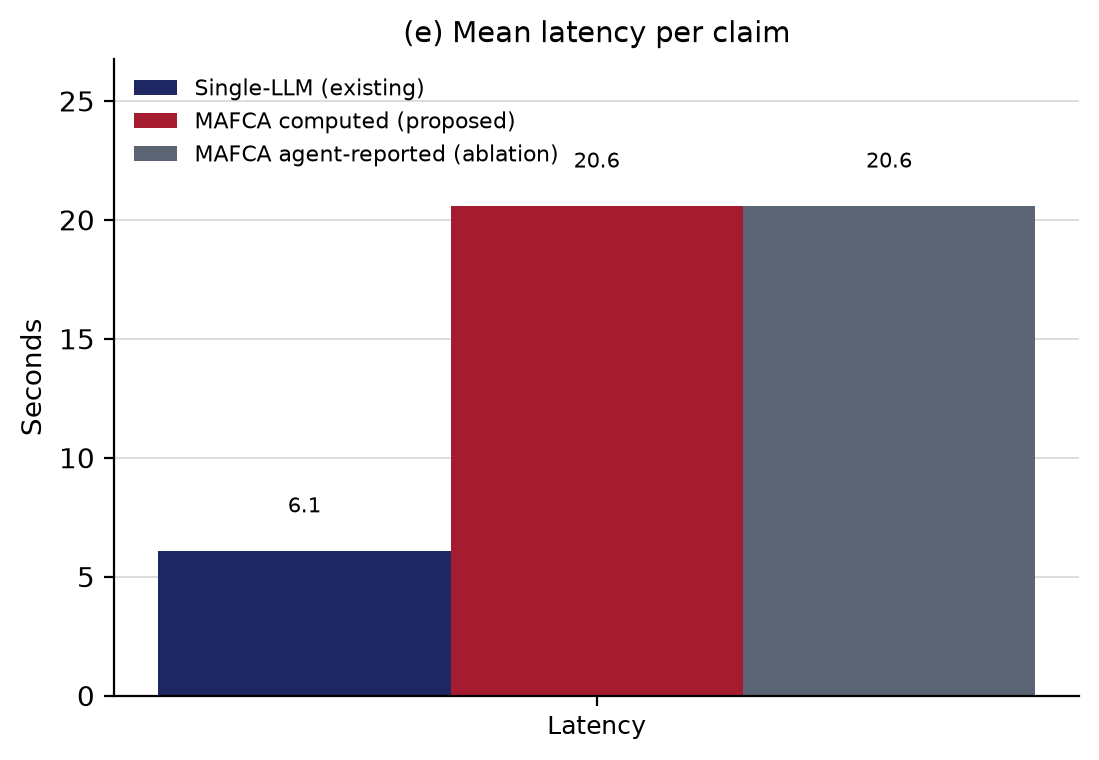
\includegraphics[width=0.84\textwidth]{figures/av_latency.png}
\caption{Mean wall-clock latency per claim. Decomposition costs time. \textit{Generated by src/analysis/results\_report.py.}}
\end{figure}
\begin{figure}[H]
\centering
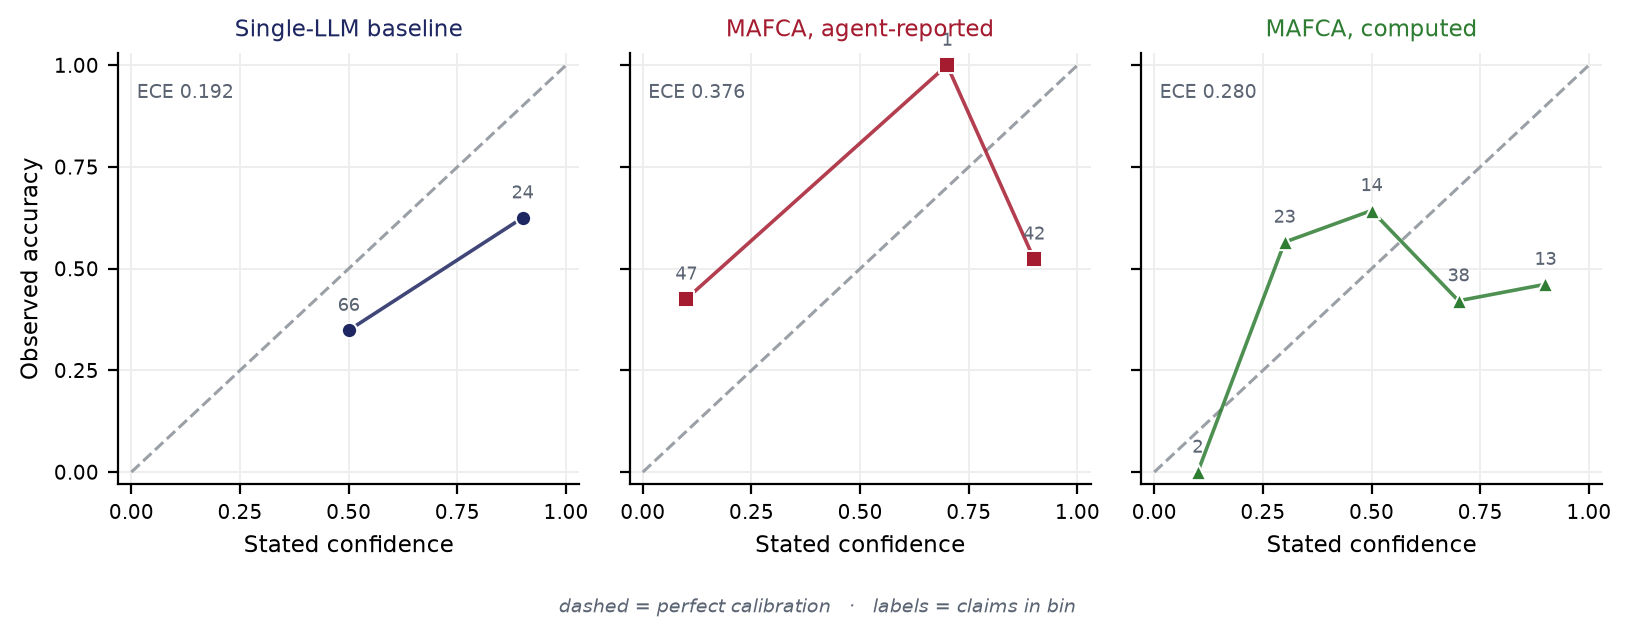
\includegraphics[width=0.84\textwidth]{figures/av_reliability.png}
\caption{Reliability diagram. A perfectly calibrated system would track the diagonal; distance from it is miscalibration. \textit{Generated by src/analysis/grounding\_figures.py.}}
\end{figure}
\begin{figure}[H]
\centering
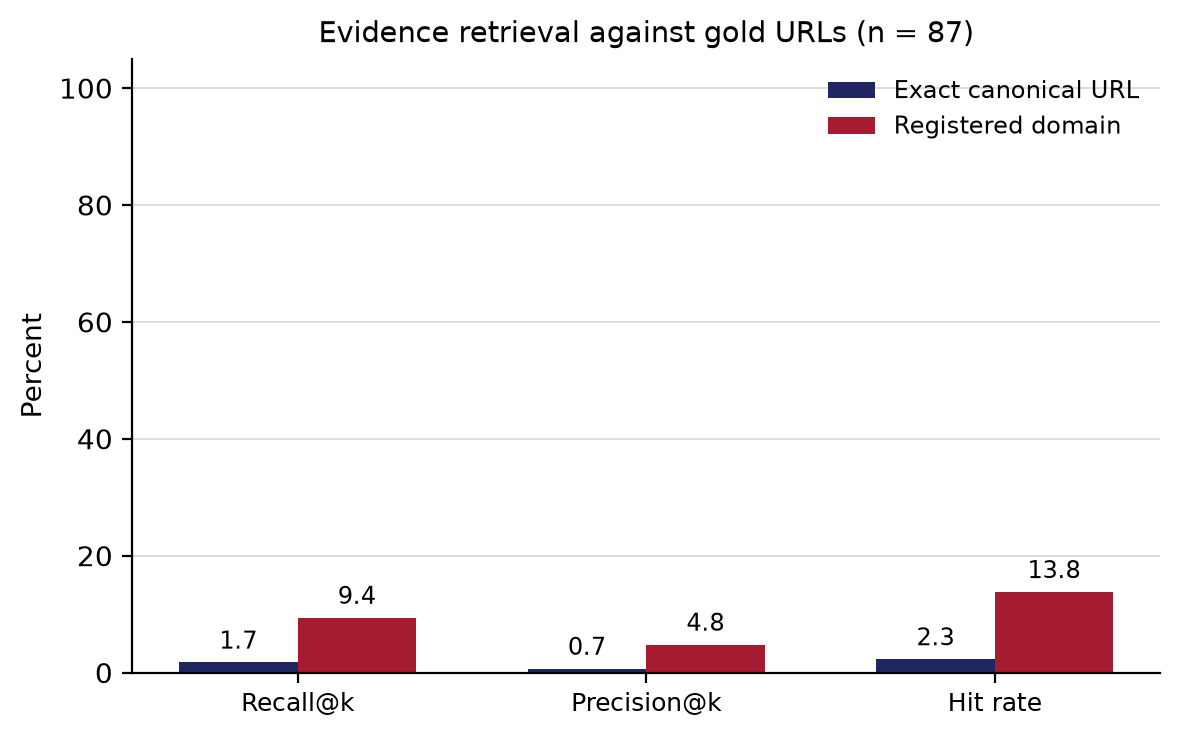
\includegraphics[width=0.84\textwidth]{figures/av_retrieval.png}
\caption{Evidence retrieval measured against the corpus' annotated gold URLs, at exact-URL and domain matching strictness. \textit{Generated by src/analysis/grounding\_figures.py.}}
\end{figure}
\begin{figure}[H]
\centering
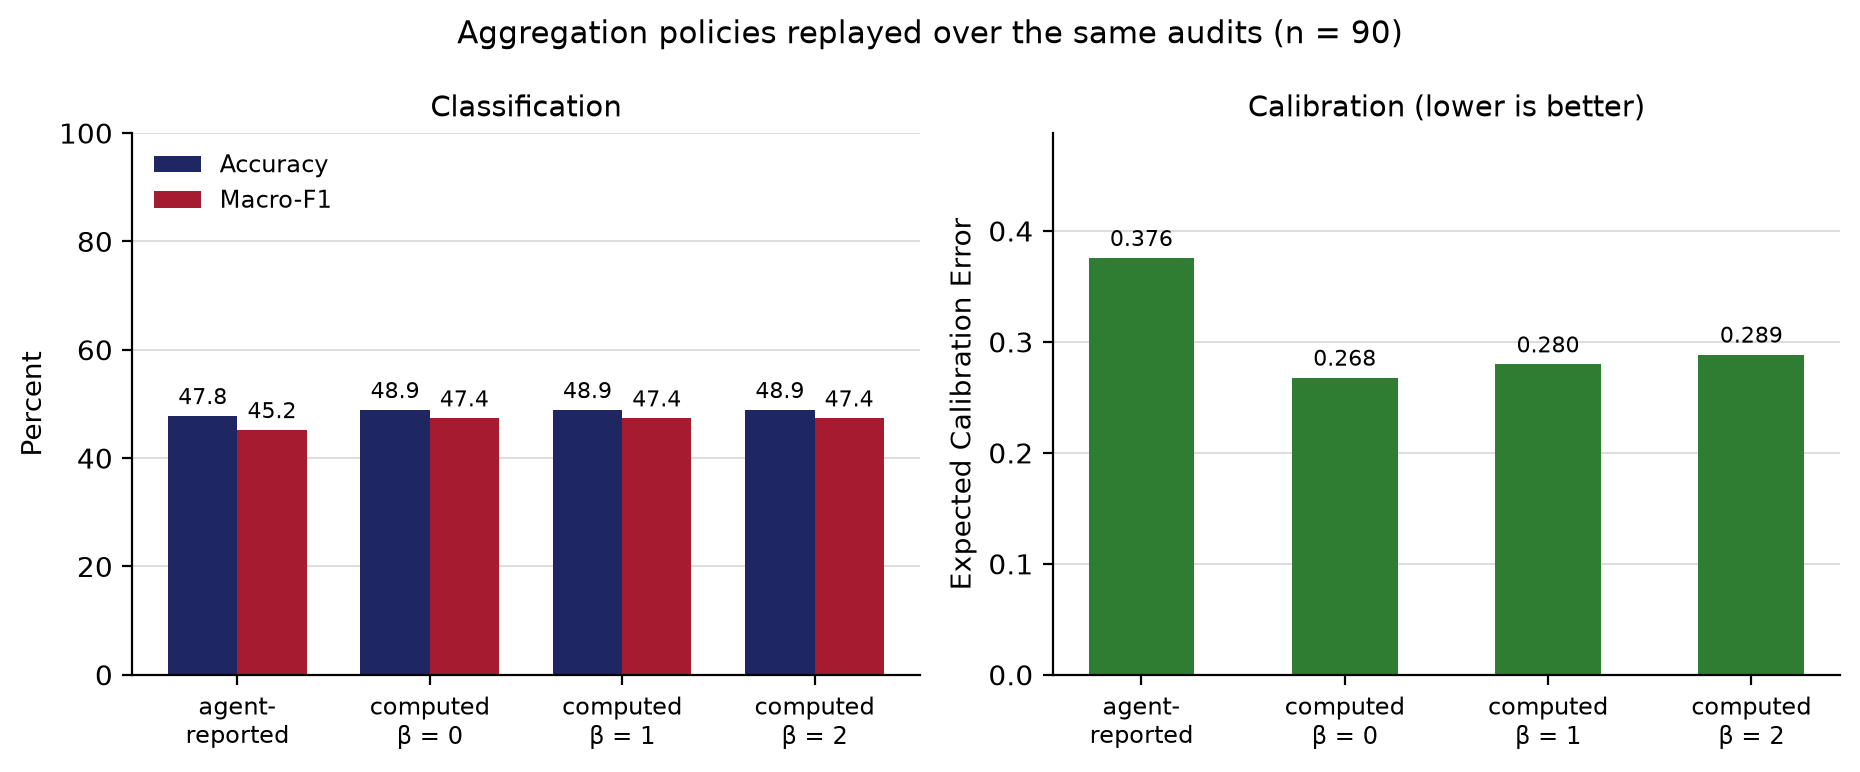
\includegraphics[width=0.84\textwidth]{figures/av_ablation.png}
\caption{Aggregation ablation over the evidence-strength weight $\beta$, which controls how much a passage's assessed strength scales its vote. \textit{Generated by src/analysis/ablation.py.}}
\end{figure}
\begin{figure}[H]
\centering
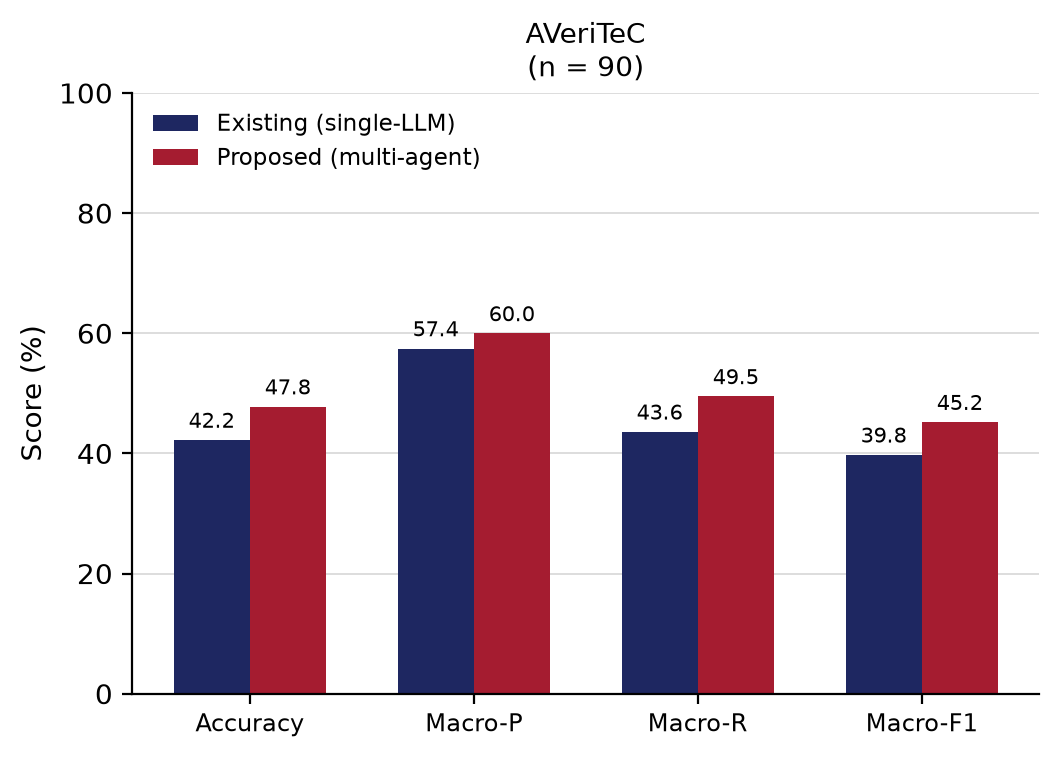
\includegraphics[width=0.84\textwidth]{figures/fig_summary_bar.png}
\caption{Summary comparison across the headline measures. \textit{Generated by src/analysis/summary\_figures.py.}}
\end{figure}
\begin{figure}[H]
\centering
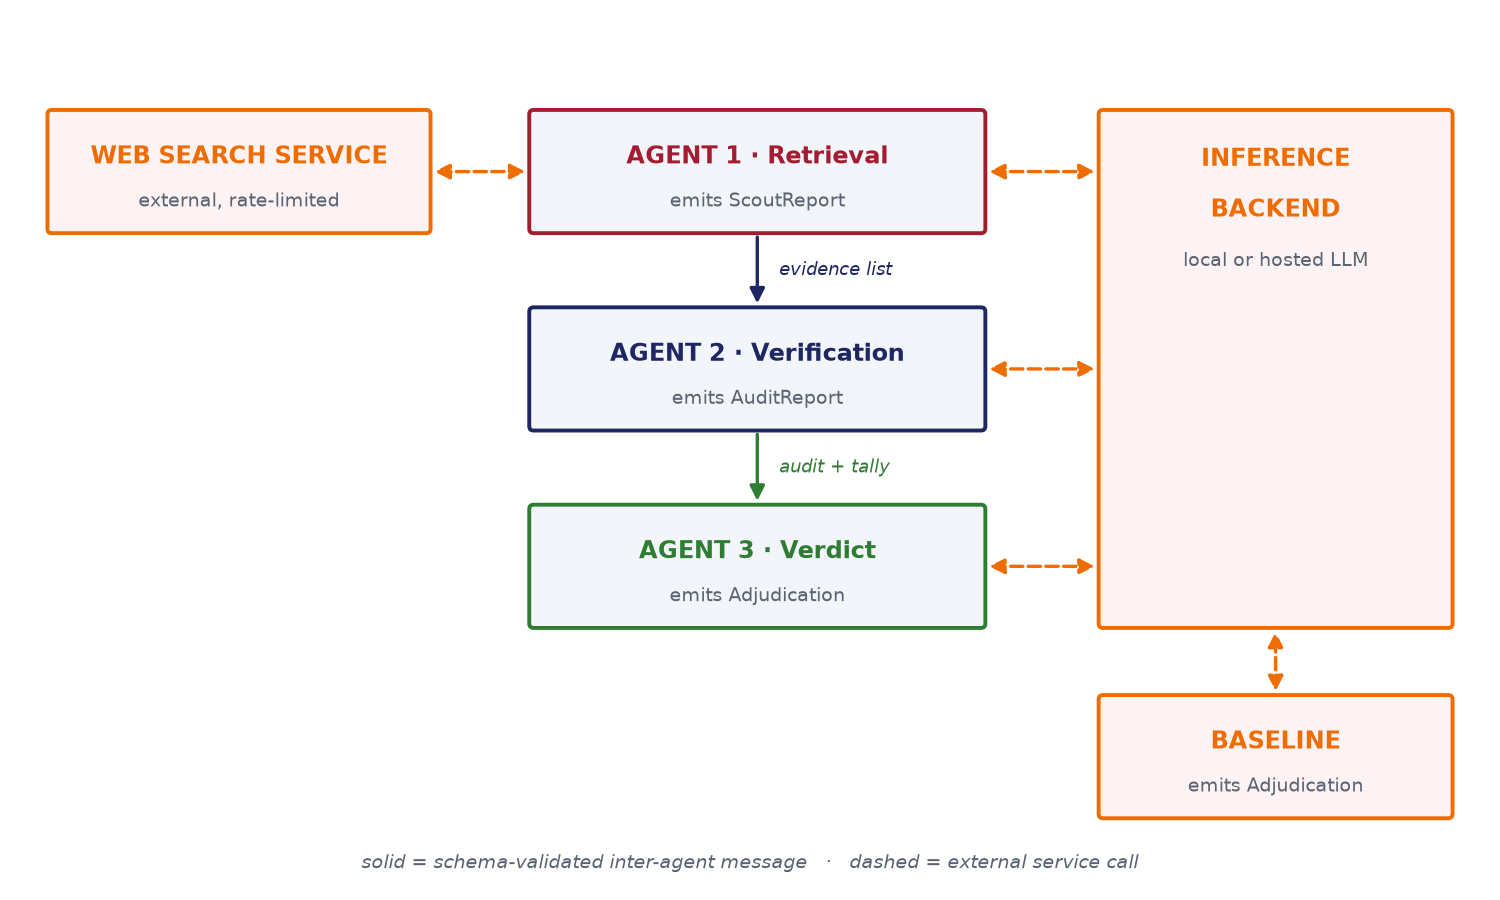
\includegraphics[width=0.84\textwidth]{figures/fig_network.png}
\caption{Agent communication structure and the typed schemas carried across each boundary. \textit{Generated by src/analysis/summary\_figures.py.}}
\end{figure}
\clearpage
\section*{Index of generated quantities}
This document draws on 510 generated macros across three files in results/macros/: numbers.tex, condition\_numbers.tex and attribution\_numbers.tex. Each is written by the analysis scripts and regenerated by src/analysis/regenerate.py.
\end{document}